\documentclass[fleqn,10pt]{olplainarticle}
% Use option lineno for line numbers 
\usepackage{cite}
\usepackage{caption}
\usepackage{subcaption}
%\usepackage[numbers,sort&compress]{natbib}
\usepackage{hyperref}
\hypersetup{colorlinks = true, urlcolor=blue, filecolor=blue, citecolor = black,linkcolor=black}

\title{CS 6000 Journal: Week 3}

\author{Minhajul Alam Rahat}
\affil{University of Colorado Colorado Springs}
\affil{\textit{mrahat@uccs.edu}}


\keywords{CS 6000, journal, coursework, survey browse, critical read, creative read}

\begin{abstract}
This journal includes searching, browsing, scanning and critical reading of survey papers which is done as part of course work in Introduction to Computer Science Research (CS 6000) .
\end{abstract}

\begin{document}

\flushbottom
\maketitle
\thispagestyle{empty}

\section{Learning/Process Followed}

I browsed survey papers related partially/fully to my research topic using Google scholar keywords. Using the metric feature decided which conference/journal I should choose. I used zotaro to add a number of surveys and later classified them to decide which papers I would consider for this journal. Reading the surveys let me understand some existing overall work in IoT security field and also some limitations and lacking in my topic. It also helped gaining perspective about the structure of a good survey paper. 
 

\section{Research Direction}

My initial research direction is IoT firmware security. I am particularly interested in analyzing techniques of IoT firmware.


\section{Critical/Creative Read}
From browsed five surveys \cite{1},\cite{2},\cite{3},\cite{4} and \cite{5} critical/creative notes for four of them are given below:

\subsection{note for \cite{1}}

They focused on the works related to IoT vulnerabilities. Started by reviewing surveys in IoT field and discussed their contributions within two classes: i) IoT architecture, technology and ii) IoT security. The first part did not shed any necessary insight about IoT vulnerability in terms of architecture/technology but the second one presented some good existing surveys on IoT security, summary of contributions and stated the lack of IoT vulnerability related survey which strengthened the stance of this work.  Their summary of vulnerability research works is categorized in nine classes, some of them are \textbf{related to my work}. They provided a good taxonomy of IoT vulnerability and classified different aspects of this taxonomy in a systematic way in terms of components, security impact, countermeasures, attacks, and situation awareness capabilities. In each category of research, they provided summary as well as their own findings about gaps/future research directions. They gave comprehensive research directions based on the analyzed lacking in existent research works. Has more citations because it classifies IoT vulnerability research into a broad classes of work with insights/directions for each of them. 

\subsection{note for \cite{2}}

The work started by describing IoT architecture, components (hardware,software) and a summary of attack surfaces. Classification of attack surfaces captured a holistic view of different boundaries for attack. They divided the survey based on four categories: i) basic framework analysis approaches, talks about some dynamic analysis framework  ii) vulnerability discovery based on dynamic and static analysis, presented a summary table of existing works (not comprehensive? limitations?), iii) vulnerability detection using network scan and code similarity analysis (noted: lack of similarity analysis work in IoT field? could be a direction of work?) (provides some good background of binary similarity), iii) vulnerability mitigation (lack of automatic patch generation work in IoT?) --- good background and evaluation presented for the given works based on technical requirement, applicable architecture, and OS. Presented some challenges in vulnerability research work and some directions. Comparing with \cite{2}, this work has small coverage of vulnerability research work -- which is the reason for less citation but for a more targeted researchers it gives comprehensive summary.

\subsection{note for \cite{3}}
Good introduction to the importance of firmware security analysis, current state of affairs in this topic. Presented reviews for firmware security, and assessment methods. Covers important IoT firmware questions in the work (table:2). Detailed structure maintained while classifying papers (table:3 -- is there any lacking?) Talks about vulnerabilities in IoT firmware and illustrates a systematic taxonomy on vulnerability, analysis tools (can use for my work), and research directions. Does not mention cross-architecture analysis? Scalable methodology? (a possible gap?) (any works on firmware other than Linux-based??) Detailed challenges and directions not present?

\subsection{note for \cite{4}}

Presents hardware based firmware extraction (focuses only on extraction methodologies, a first step of firmware analysis). Describes different firmware extraction processes and presents a case study for various platforms. Concludes by giving some countermeasures. Does a good job on giving an elaborate methodologies existent in firmware extraction field, and published an open source repository containing the information about analyzed device. Is it important for my work ? --- might shed some light on preliminary extraction. Does not give any structured taxonomy, detailed existing research or limitations. 

\section{Topic Map}

The number of surveys in IoT firmware analysis is still low. From the surveys found during browsing, some possible gaps can be stated regarding IoT firmware analysis and security. The gaps are summarized in \ref{fig:my_label}. In this field we can do an exhaustive study of existing methodologies regarding IoT firmware analysis. We can try to find answers if exist for some questions like: how can we improve the analysis algorithm? Is there any feasible methods of analysis that can be used in different IoT architecture? Is there any scalable technique we can use for vulnerability discovery? Is there any large scale study for firmware images that can be used to narrow down common security issues in different devices, is there any security standard that can be implemented for threat mitigation?

\section{Github Link}
\appendix

The link to the latex source code is: \url{https://github.com/Minhaj-Rahat/CS6000-journal3-}

\begin{figure}[h]
    \centering
    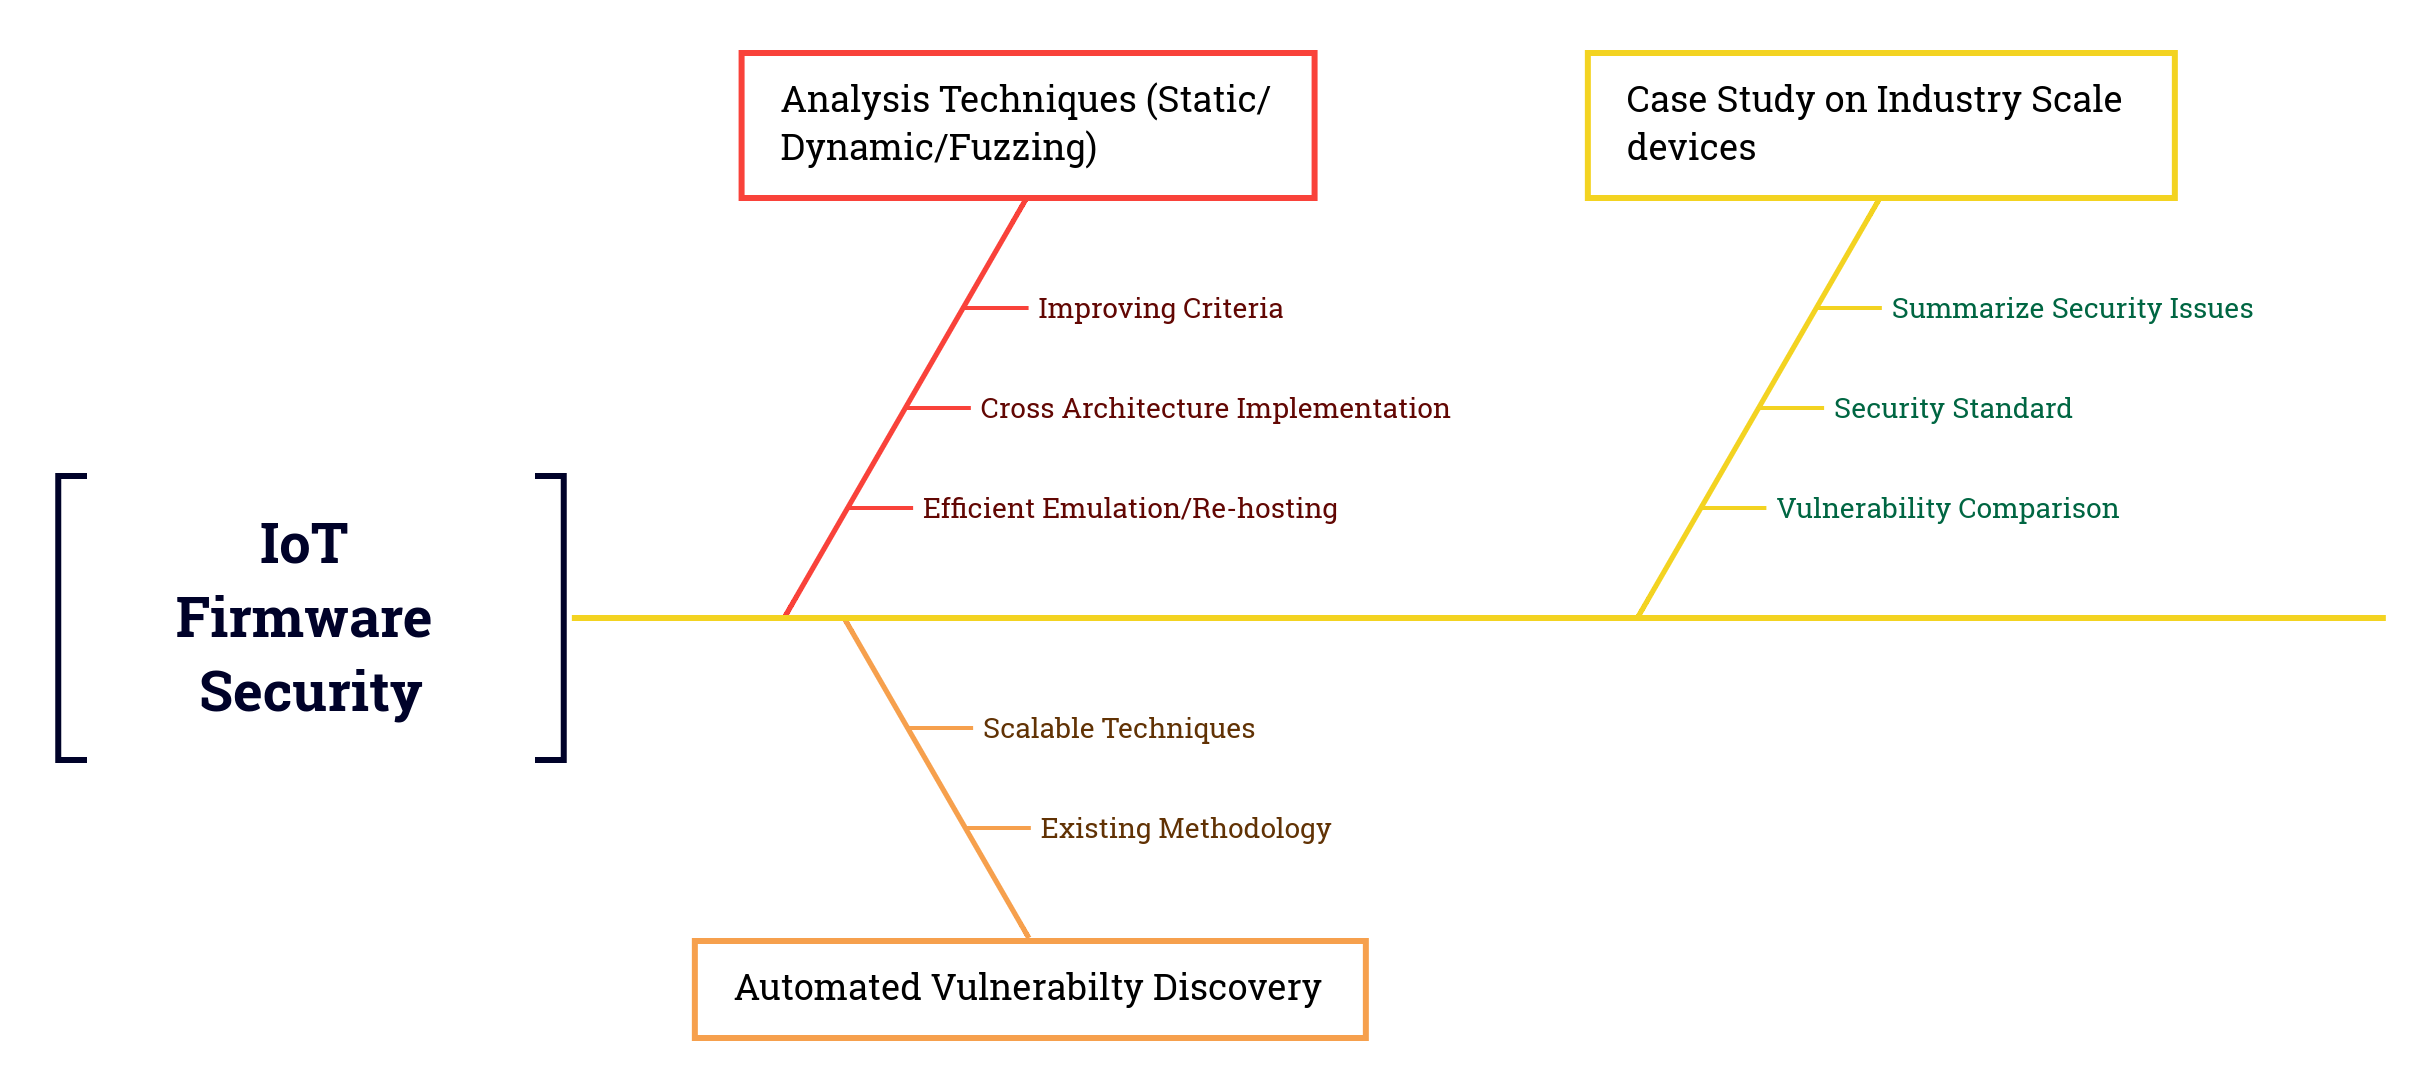
\includegraphics[width=1\linewidth]{IoT Firmware Security.png}
    \caption{Topic Map for Future Work}
    \label{fig:my_label}
\end{figure}

\clearpage

\bibliographystyle{IEEEtran}
\bibliography{main}



\end{document}